
%|  Name  | TODO | ONGOING | DONE |
%|--------|------|---------|------|
%| Dana   | x    |         |      |
%| Gerd   |      |         |  x   |
%| Glenn  | x    |         | x    |
%| Jordan | x    |         |      |
%| Luke   | x    |         |      |
%| Matt   |      |         | x    |
%| Neil   | x    |         |      |
%| Scot   | x    |        |   x   |

This document is intended to provide a detailed and in-depth understanding of how the HDF5 library operates. It delves into the underlying principles of the library and examines its systemic, structural, and orderly aspects responsible for its clear and informative functioning. Anyone going through this document can gain valuable insights into the library’s architecture and learn how to use it efficiently. Furthermore, it provides an overview of various techniques that can be used to simplify the understanding of the operations of the HDF5 library, making it easier to work with and more accessible for users of all levels of expertise.

\section{Audience and Goals}

This document aims to help readers achieve the outcomes they want. Such readers might be

\begin{itemize}
    \item Community contributors looking for guidance in addressing issues
    \item New library developers trying to find their bearings in a large code base
    \item HDF5 library extension developers who want to ``dig deeper"
    \item HDF5 power users who want to understand ``how the library really works.''
\end{itemize}

While comprehensiveness (= covering a wide range of topics related to a subject) is one of the goals for this document, completeness (= having all necessary parts) is not, at least not for this version. While helping readers achieve outcomes is the purpose of this document, it is not focused on specific tasks and is not a ``cookbook.''

We have organized the material in two parts: a set of guided tours (Chapter \ref{part:tours}) and a reference (Chapter \ref{part:reference}). The guided tours provide specific contexts where subsets of architectural concerns can be discussed. The reference is ``context-free'' in the sense that each topic can be consulted and stands on its own.

\section{Architecture}

Architectural documentation of a system or software consists of a set of models for an audience. Different models represent different perspectives or views of, in this case, the HDF5 library. One of the perhaps simplest models of the HDF5 library is shown in Figure~\ref{fig:blackbox}.

\begin{figure}[ht]
\centering
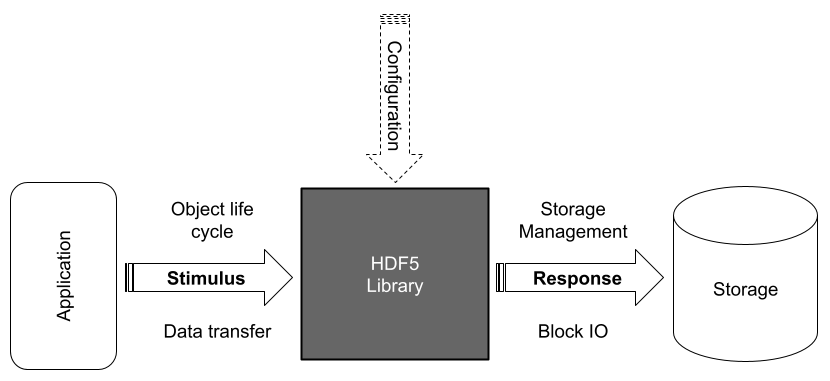
\includegraphics[width=0.9\textwidth]{images/Black box.png}
\caption{A black box model of the HDF5 library.}
\label{fig:blackbox}
\end{figure}

Despite its simplicity, a black box model gives us context for other models and lets us ask relevant questions. One of its central premises is that by correlating stimuli and responses, we might be able to draw certain conclusions about the black box's ``inner workings." However, it is not straightforward to correlate HDF5 API calls with actual IO activity. This is the case for three reasons:
\begin{enumerate}
    \item The HDF5 library is an intermediate abstraction layer
    \item It (de-)serializes collections of complex object constellations into storage structures
    \item IO activity occurs in blocks.
\end{enumerate}
Hence, we must open the box, which is what this document is about.

The stimuli to which we can subject the black box come in two forms: object life cycle management instructions and data transfer requests. Object life cycle management means tasks such as creating and modifying familiar HDF5 objects (datasets, groups, datatypes). By data transfer, we mean any kind of \texttt{*read*} or \texttt{*write*} API call, which is intended to transfer user (meta-)data into storage.

The black box responds to stimuli in two forms: storage management and block IO operations. Typical examples of storage include file systems and object stores. Specific responses depend on how HDF5 data model primitives are encoded in storage primitives. Examples include single- or multi-file layouts or collections of storage objects.

When observing the stimulus/response ``traffic" of even simple applications, the correlation is much weaker and less direct than we might expect and sometimes outright counter-intuitive (e.g., an input operation triggering an output operation). Unlike a mathematical function, which consistently produces the same outputs for the same inputs, the relation between stimuli and responses exhibited by the HDF5 library is non-functional, albeit deterministic. This is due to the HDF5 library's role as a translator between HDF5 model idioms, represented in memory, and storage idioms. To be effective and efficient, and to bridge the speed differential between memory and storage, the HDF5 library maintains a state. This state dilutes the simple stimulus/response logic and manifests itself in what might appear as a delayed response or an aggregate response to a sequence of stimuli.

The architecture of a system or software is usually presented in models that fall under different perspectives or views, such as the ones shown in Table~\ref{table:perspectives}.

\begin{table}[h!]
\begin{tabular}{||c|l||}
\hline
Perspective or View & Description \\  [0.5ex] 
\hline\hline
Purpose/objective & What the client wants \\  
Form & What the system is \\
Behavioral or functional & What the system does\\
Performance objectives or requirements & How effectively the system does it\\
Data & The information retained in the system and its relationships\\
Managerial & The process by which the system is constructed and managed\\ [1ex] 
\hline
\end{tabular}
\caption{Six common perspectives or views.~\cite{maier2009}}
\label{table:perspectives}
\end{table}

For a given system or software, not all of them are equally important or relevant at all times. For example, the library build process and testing (managerial view) is covered in the first guided tour, whereas the modular library structure (functional view) is the organizing principle for the reference.

\section{Purpose, Objectives, and Values}

The purpose of the \acrshort{hdf5} library is to ensure efficient and equitable access to science and engineering data stored in HDF5 files across platforms and environments, now and forever. Toward that purpose, the two main objectives are:

\begin{enumerate}
    \item Self-describing data
    \item Portable encapsulation and access
\end{enumerate}

Self-describing data captures all information about itself necessary to reproduce and interpret it as intended by its producer. A storage representation must preserve the self-describing nature when transferring such representations over a network or to different storage. At the same time, it should be accompanied by a portable library that allows applications to access the data without knowing anything about the details of the representation.

The ``marriage''~\cite{kuehn1996} of the HDF5 file format and library is a specific implementation of the primitives and operations defined by the HDF5 data model and was adapted for several specific use cases over time.

\begin{figure}[ht]
\centering
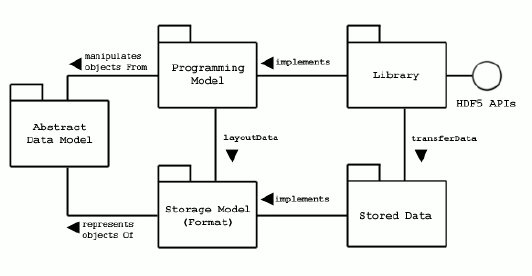
\includegraphics[width=0.7\textwidth]{images/models.png}
\label{fig:img1}
\caption{Models}
\end{figure}

The implementation is guided by the following values, which are listed in no particular order.

\begin{description}
    \item[Extensibility] The degree to which users can change behavior and appearance.
    \begin{itemize}
        \item Datatypes, conversions
        \item Filters
        \item Links
        \item Data virtualization
        \item Storage types
        \item File format micro-versioning
    \end{itemize}
    \item[Compatibility, Longevity, \& Stability] Things that worked before continue to work the same indefinitely
    \begin{itemize}
        \item Quasi-static data model
        \item Backward- and forward compatibility
        \item API Versioning
        \item Open file format specification
    \end{itemize}
    \item[Efficiency] Effective operation as measured by comparing production with cost (as in time, storage, energy, etc.)
    \begin{itemize}
        \item Algorithmic complexity
        \item Scalability
    \end{itemize}
    \item[Maintainability] The degree to which it can be modified without introducing fault
    \begin{itemize}
        \item Additive software construction~\cite{hanson2021}
    \end{itemize}
    \item[Progressiveness] A measure of eagerness to make progress and leverage modern storage technology
    \item[Freedom] Specifically, free software means users have the four essential freedoms~\cite{fsf2023}
    \begin{itemize}
        \item The freedom to run the program as you wish, for any purpose (freedom 0).
        \item The freedom to study how the program works, and change it so it does your computing as you wish (freedom 1). Access to the source code is a precondition for this.
        \item The freedom to redistribute copies to help others (freedom 2).
        \item The freedom to distribute copies of your modified versions to others (freedom 3). By doing this, you can give the whole community a chance to benefit from your changes. Access to the source code is a precondition for this.
    \end{itemize}
\end{description}

\section{How this document is organized}

This document has three parts. Part one is a set of guided tours that are used to uncover architectural elements, but without going into too much detail. The second part, currently a fragment, is meant as a reflection on problems in the HDF5 library architecture. Part three is a reference section, where specific architectural elements are explored in greater detail, in some cases, for the first time, in non-source code form.

\section{Typographic conventions}

\begin{itemize}
    \item[\textbf{bold}] headers, titles
    \item[\textit{italic}] emphasis
    \item[\texttt{monospace}] source code, package names, configuration file settings, file system paths and folder names.
\end{itemize}